\chapter{Fejlesztői dokumentáció}
\label{ch:impl}

A program számos segítséget ad fejlesztőknek a kód egyszerű értelmezésére; a kód bővítésére. Vállalkozó szellemű embereknek a program egy teljes Java interpretert tud nyújtani viszonylag kevés továbbfejlesztéssel. A Java bájtkód instrukciók megértése során bármely Java fejlesztő jobban tudja értékelni, hogy mit is csinál a Java fordítóprogram a háttérben. A program nagyon szorosan épül a JVM specifikációra, a specifikációt annak megfelelően próbálja implementálni.

\section{Probléma specifikációja}

A probléma egy fájl beolvasásával kezdődik. Minden class fájl legelején szerepel a \lstinline{CA FE BA BE} konstans bájt sorozat. Ez egy szükséges, viszont nem elégséges feltétel egy class fájl érvényességére. A konstans értéken felül számos más értéket is tartalmaz egy class fájl. Ha ezek a specifikációnak megfelelően vannak, és a fájl végén nincsen extra bájt, akkor érvényes ténylegesen a class fájl.

Ebben a class fájlban, ha érvényes, megpróbáljuk a belépési pont függvényét megkeresni. Ez Java programokban a \lstinline{main} függvény.

Ehhez a függvényhez tartozik egy bájt sorozat a class fájlban, amely a függvény során végrehajtandó tényleges utasítások bájt sorozata. A probléma megoldására nekünk ezt a sorozatot szükséges értelmeznünk. Ha a bájt sorozat megköveteli, akkor más függvényeket kell meghívnunk, amelyek lehetnek ugyanabban a fájlban, viszont lehet hogy más fájlban vannak benne, ilyenkor szükséges egy másik class fájlt beolvasnunk, majd a megfelelő függvényt értelmeznünk.

A probléma megoldására során minden hibát szeretnénk a felhasználó felé megfelelően továbbítani, példa ezekre:
\begin{compactitem}
	\item A megadott class fájl nem érvényes
	\item A megadott class fájl nem tartalmaz érvényes belépési pontot
	\item A belépési pont futtatása során hiba keletkezett
\end{compactitem}

Természetesen ugyanígy a sikeres futást is szeretnénk a felhasználó felé továbbítani. A sikeres futás itt azt jelenti, ha a kimenet megyezik a beépített \lstinline{java} interpreter kimenetével.

\section{Megoldás lépései}

\subsection{Class fájl felépítése}

A specifikáció alapján a class fájl felépítése a következő:

\begin{compactitem}
	\item 4 bájt konstans bájt sorozat (\lstinline{CA FE BA BE})
	\item 2 bájt \lstinline{minor} verziószám
	\item 2 bájt \lstinline{mayor} verziószám
	\item 2 bájt \lstinline{Constant Pool} darabszáma (+1, az 1-től való indexelés miatt)
	\item Változó bájt \lstinline{Constant Pool Info} (praktikusan amíg darabszámnyit nem tudtuk beolvasni)
	\item 2 bájt hozzáférési zászlók
	\item 2 bájt a \lstinline{this} osztály indexére
	\item 2 bájt a \lstinline{super} osztály indexére (minden osztály valamely osztály leszármazottja)
	\item 2 bájt az interfészek darabszáma
	\item Változó bájt interfész információ
	\item 2 bájt a függvények darabszáma
	\item Változó bájt függvény információ
	\item 2 bájt az osztály attribútumainak darabszáma
	\item Változó bájt osztály attribútum információ
\end{compactitem}

\subsubsection{Class fájltól a benne levő metódus futtatásáig}

A fő osztály a \lstinline{ClassFile}, amely számos dologért felel. Többek között egy class fájl beolvasáért, amely során a megfelelő adattagok beállítja. A \lstinline{ClassFile} osztálynak egy konstruktora van, mégpedig:
\begin{minted}{java}
public ClassFile(String fileName)
\end{minted}
Tehát az egyetlen paraméter a beolvasandó class fájl neve.

A konstruktor meghívása egyidejüleg meghívja a \lstinline{readClassFile} függvényt is:
\begin{minted}{java}
public void readClassFile(String fileName)
\end{minted}
Ez a függvény egy adott fájlnévre beolvassa a class fájlban tárolt adatokat a megfelelő változókba.
(Ezen felül egy \lstinline{VALID_CLASS_FILE} változót is beállít; feltétellezük hogy ha a mágikus szám \lstinline{(CA FE BA BE)} megtalálható a fájl elején, akkor az adott fájl egy valid class fájl, ellenkező esetben egy \lstinline{InvalidClassFileException}-t dob a beolvasó függvény.)

A beolvasás után (tehát az objektum létrehozása után) érdemes a belépési függvényt (általában \lstinline{main}) megkeresni a \lstinline{findMethodsByName} metódussal:
\begin{minted}{java}
public Method_Info findMethodsByName(String methodName, String methodDescription)
\end{minted}
Ez egy adott függvénynévre a megfelelő nevű metódust visszaadja a beolvasott fájlból (ha nem talál ilyet akkor \lstinline{null}-t ad vissza). 

Opcionális paraméterként megadhatjuk a metódus szignatúráját is, ehhez a JVM specifikációban szereplő típus szöveggé való kódolásának mintája használandó.
\begin{table}[H]
	\centering
	\begin{tabular}{ | m{0.25\textwidth} | m{0.65\textwidth} | }
		\hline
		\textbf{Kódolt típus} & \textbf{Java Típus} \\
		\hline \hline
		B & byte \\
		\hline
		C & char \\
		\hline
		D & double \\
		\hline
		F & float \\
		\hline
		I & int \\
		\hline
		J & long \\
		\hline
		L\textit{classnév}; & reference (osztály) \\
		\hline
		S & short \\
		\hline
		Z & boolean \\
		\hline
		{[} & reference (tömb) \\
		\hline
	\end{tabular}
	\caption{Típust tartalmazó szöveg dekódolásá Java típusokká a JVM specifikáció alapján}
	\label{tab:jvmtypeencoding}
\end{table}

A bemeneti paramétereket zárójelek választják el, ezután szerepel a visszatérési érték. Tehát az általános Java belépési függvény, a \lstinline{main} java kódja:
\begin{minted}{Java}
public static void main(String[] args)
\end{minted}
Ennek a függvény szignatúrájának kódolása a következő: \lstinline{([Ljava/lang/String;)V}

Példa a belépési metódust megkereső függvény használatára:
\begin{minted}{java}
ClassFile CLASS_FILE = new ClassFile("Main.class");
Method_Info method = CLASS_FILE.findMethodsByName("main", "([Ljava/lang/String;)V");
\end{minted}

A függvény megtalálása után ajánlott a \lstinline{Code} attribútumot megtalálni, ebben, többek között, található a futtatandó Java bájtkód is. A segédfüggvény erre a \lstinline{findAttributesByName}:
\begin{minted}{java}
public List<Attribute_Info> findAttributesByName(List<Attribute_Info> attributes, String attributeName)
\end{minted}
Mivel egy attribútumból több is lehet, egy listát kapunk vissza (a \lstinline{Code}-ból csak egy lesz), bemeneti paraméterként az attribútumnév mellett a megfelelü függvény attribútumait is át kell adnuk, például:
\begin{minted}{java}
List<Attribute_Info> attributes = CLASS_FILE.findAttributesByName(method.attributes, "Code");
\end{minted}
(Ha nem talál ilyen nevezetű attribútumot akkor üres listát ad vissza.)

A megfelelően beolvasott attribútum után, a megtalált attribútumok között ajanlott végigmenni, a \lstinline{List} implementálja az \lstinline{Iterable}-t, így egy for ciklussal elegánsan megtehetjük ezt:
\begin{minted}{java}
for (Attribute_Info attribute : attributes)
\end{minted}

Mivel \lstinline{Code} attribútumokról beszélünk, ezért a következő ajánlott dolog hogy ebből az attribútumból olvassuk be az adatokat. Ehhez a \lstinline{Code_Attribute_Helper} osztály \lstinline{readCodeAttributes} metódusa megfelelő:
\begin{minted}{java}
public static Code_Attribute readCodeAttributes(Attribute_Info attribute) throws IOException
\end{minted}
A függvény egy attribútumot vár (például az előbbi kódrészlet \lstinline{attribute} változóját), majd pedig beolvassa a specifikációnak megfelelően a \lstinline{Code_Attribute}-ot, és visszaadja azt, ha valamiért nem sikerült a beolvasás, akkor \lstinline{IOException}-t dob a függvény.
\begin{minted}{java}
Code_Attribute codeAttribute = Code_Attribute_Helper.readCodeAttributes(attribute);
\end{minted}

Ezt a beolvasott attribútumot a \lstinline{ClassFile} osztály fel tudja használni az \lstinline{executeCode} metódusával, mely egy \lstinline{byte[]} változót vár bemeneti paraméterként, ami a \lstinline{Code_Attribute} része:
\begin{minted}{java}
public Pair<Class<?>, Object> executeCode(byte[] code, Object[] args) Throwable
\end{minted}
A reflekció miatt számos hibát dob vissza a függvény, ha nem helyes a kód formátuma akkor \lstinline{IOException}-t dob a függvény, viszont egy \lstinline{Throwable}-el az egészet le tudjuk kezelni; a \lstinline{Throwable} az \lstinline{ATHROW} Java bájtkód instrukció miatt egyébként szükséges (ekkor egy hibát dob vissza a metódusunk).
Visszatérési értéke \lstinline{Pair<Class<?>, Object>}, a számos \lstinline{RETURN} utasítás miatt (ezeket a \lstinline{stack}-en szükséges elhelyeznünk).
Opcionálisan megadhatunk neki egy \lstinline{args}-ot is, amely a függvény paramétere(i) egy \lstinline{Object} tömbben.
Példa a használatára:
\begin{minted}{java}
CLASS_FILE.executeCode(codeAttribute.code, null);
\end{minted}

Ezzel el is jutottunk egy class fájl beolvasásától, az abban lévő adott függvény Java bájtkódjának futtatásáig, több teendőnk nincsen, a program az adott függvényben levő külön függvényhívásokat automatikusan elvégzi.

\begin{listing}[H]
A teljes példakód:
\begin{minted}{java}
public class Interpreter {
	public static void main(String[] args) throws Throwable {
		ClassFile CLASS_FILE = new ClassFile("Main.class");
		Method_Info method = CLASS_FILE.findMethodsByName("main", "([Ljava/lang/String;)V");
		List<Attribute_Info> attributes = CLASS_FILE.findAttributesByName(method.attributes, "Code");

		for (Attribute_Info attribute : attributes) {
			Code_Attribute codeAttribute = Code_Attribute_Helper.readCodeAttributes(attribute);
			CLASS_FILE.executeCode(codeAttribute.code, null);
		}
	}
}
\end{minted}
\caption{Példa a Main.class interpretálására}
\end{listing}

\subsubsection{Pár minta class fájl felépítésére}

A legegyszerűbb class fájl ami értelmes, viszont nem futtattható:

\begin{center}
\begin{tabular}{ c c c c c c c c c c c c c c c c }
\stagemagic{CA} & \stagemagic{FE} & \stagemagic{BA} & \stagemagic{BE} & \stageminor{00} & \stageminor{00} & \stagemajor{00} & \stagemajor{00} & \stageconstantsize{00} & \stageconstantsize{00} & \stageaccessflags{00} & \stageaccessflags{00} & \stagethisclass{00} & \stagethisclass{00} & \stagesuperclass{00} & \stagesuperclass{00} \\
\stageinterfacesize{00} & \stageinterfacesize{00} & \stagefieldsize{00} & \stagefieldsize{00} & \stagemethodsize{00} & \stagemethodsize{00} & \stageattributes{00} & \stageattributes{00}
\end{tabular}
\end{center}


\begin{listing}[H]
Java kódban ennek megfelelője az üres fájl:
\begin{minted}{java}
\end{minted}
\caption{Legegyszerűbb class fájl Java kódja}
\end{listing}

Elérhető a \lstinline{src/test/java/com/zoltanbalazs/Simple.class} fájl formátumában

class fájl formátumának magyarázata:

\begin{compactitem}
\setlength\itemsep{-5px}
\item \stagemagic{CA FE BA BE}: Mágikus szám, amely minden class fájl elején megtalálható
\item \stageminor{00 00} \stagemajor{00 00}: class fájl \lstinline{Minor} és \lstinline{Major} verziószáma, egy táblázatnak megfelelően a fordítóprogram verziója
\item \stageconstantsize{00 00}: A \lstinline{Constant Pool} mérete (+1, mivel 1-től indexelt, itt nem számít)
\item \stageaccessflags{00 00}: Az osztály hozzáférési zászlói ()
\item \stagethisclass{00 00}: \lstinline{This} osztály indexe a \lstinline{Constant Pool}-ban
\item \stagesuperclass{00 00}: \lstinline{Super} osztály indexe a \lstinline{Constant Pool}-ban
\item \stageinterfacesize{00 00}: Interfészek száma (00 00\textsubscript{16} = 0\textsubscript{10} db)
\item \stagefieldsize{00 00}: Adattagok száma (00 00\textsubscript{16} = 0\textsubscript{10} db)
\item \stagemethodsize{00 00}: Függvények száma (00 00\textsubscript{16} = 0\textsubscript{10} db)
\item \stageattributes{00 00}: Osztály attribútumainak száma (00 00\textsubscript{16} = 0\textsubscript{10} db)
\end{compactitem}

A legegyszerűbb class fájl amit a $Jabyinja$ program le tud futtatni (a beépített \lstinline{java} interpreter program nem képes ezt lefuttatni, mivel a \lstinline{main} metódus szignatúrája nem megfelelő (a paraméterek kötelezőek), illetve nincsenek osztályok):

\begin{center}
\begin{tabular}{ c c c c c c c c c c c c c c c c }
\stagemagic{CA} & \stagemagic{FE} & \stagemagic{BA} & \stagemagic{BE} & \stageminor{00} & \stageminor{00} & \stagemajor{00} & \stagemajor{00} & \stageconstantsize{00} & \stageconstantsize{04} & \stageconstantpool{01} & \stageconstantpool{00} & \stageconstantpool{04} & \stageconstantpool{43} & \stageconstantpool{6F} & \stageconstantpool{64} \\
\stageconstantpool{65} & \stageconstantpool{01} & \stageconstantpool{00} & \stageconstantpool{04} & \stageconstantpool{6D} & \stageconstantpool{61} & \stageconstantpool{69} & \stageconstantpool{6E} & \stageconstantpool{01} & \stageconstantpool{00} & \stageconstantpool{03} & \stageconstantpool{28} & \stageconstantpool{29} & \stageconstantpool{56} & \stageaccessflags{00} & \stageaccessflags{21} \\
\stagethisclass{00} & \stagethisclass{00} & \stagesuperclass{00} & \stagesuperclass{00} & \stageinterfacesize{00} & \stageinterfacesize{00} & \stagefieldsize{00} & \stagefieldsize{00} & \stagemethodsize{00} & \stagemethodsize{01} & \stagemethods{00} & \stagemethods{09} & \stagemethods{00} & \stagemethods{02} & \stagemethods{00} & \stagemethods{03} \\ 
\stagemethods{00} & \stagemethods{01} & \stagemethods{00} & \stagemethods{01} & \stagemethods{00} & \stagemethods{00} & \stagemethods{00} & \stagemethods{0D} & \stagemethods{00} & \stagemethods{00} & \stagemethods{00} & \stagemethods{00} & \stagemethods{00} & \stagemethods{00} & \stagemethods{00} & \stagemethods{01} \\
\stagemethods{B1} & \stagemethods{00} & \stagemethods{00} & \stagemethods{00} & \stagemethods{00} & \stageattributes{00} & \stageattributes{00}
\end{tabular}
\end{center}

\begin{listing}[H]
Java kód megfelelője:
\begin{minted}{java}
public static void main() {
    return;
}
\end{minted}
\caption{Legegyszerűbb class fájl, amely a szakdolgozat programja által futtatható, Java kódja}
\end{listing}

Elérhető a \lstinline{src/test/java/com/zoltanbalazs/Base.class} fájl formátumában

class fájl formátumának magyarázata:

\begin{compactitem}
\setlength\itemsep{-5px}
\item \stagemagic{CA FE BA BE}: Mágikus szám, amely minden class fájl elején megtalálható
\item \stageminor{00 00} \stagemajor{00 00}: class fájl \lstinline{Minor} és \lstinline{Major} verziószáma, egy táblázatnak megfelelően a \lstinline{javac} fordítóprogram verziója
\item \stageconstantsize{00 04}: A \lstinline{Constant Pool} mérete (+1, mivel 1-től indexelt, jelen esetben: 00 04\textsubscript{16} = 4\textsubscript{10}, 4 - 1 = 3 db)
\item \stageconstantpool{01 00 04 43 6F 64 65 01 00 04 6D 61 69 6E 01 00 03 28 29 56}: \lstinline{Constant Pool}
\begin{compactitem}
    \setlength\itemsep{-5px}
    \item \stagemajor{01} \stageminor{00 04} \stageconstantsize{43 6F 64 65} \\
    \stagemajor{01}: \lstinline{Constant Pool Info} érték \lstinline{(CONSTANT_Utf8)} \\
    \stageminor{00 04}: 00 04\textsubscript{16} = 4\textsubscript{10} hosszú \\
    \stageconstantsize{43 6F 64 65}: A \lstinline{CONSTANT_Utf8} értéke: \lstinline{Code}
    \item \stagemajor{01} \stageminor{00 04} \stageconstantsize{6D 61 69 6E} \\
    \stagemajor{01}: \lstinline{Constant Pool Info} érték \lstinline{(CONSTANT_Utf8)} \\
    \stageminor{00 04}: 00 04\textsubscript{16} = 4\textsubscript{10} hosszú \\
    \stageconstantsize{6D 61 69 6E}: A \lstinline{CONSTANT_Utf8} értéke: \lstinline{main}
    \item \stagemajor{01} \stageminor{00 03} \stageconstantsize{28 29 56} \\
    \stagemajor{01}: \lstinline{Constant Pool Info} érték \lstinline{(CONSTANT_Utf8)} \\
    \stageminor{00 03}: 00 03\textsubscript{16} = 3\textsubscript{10} hosszú \\
    \stageconstantsize{28 29 56}: A \lstinline{CONSTANT_Utf8} értéke: \lstinline{()V}
\end{compactitem}
\item \stageaccessflags{00 21}: Az osztály hozzáférési zászlói \lstinline{(Public, Super)} - elhanyagolhatóak ebben az esetben
\item \stagethisclass{00 00}: \lstinline{This} osztály indexe a \lstinline{Constant Pool}-ban
\item \stagesuperclass{00 00}: \lstinline{Super} osztály indexe a \lstinline{Constant Pool}-ban
\item \stageinterfacesize{00 00}: Interfészek száma (00 00\textsubscript{16} = 0\textsubscript{10} db)
\item \stagefieldsize{00 00}: Adattagok száma (00 00\textsubscript{16} = 0\textsubscript{10} db)
\item \stagemethodsize{00 01}: Függvények száma (00 01\textsubscript{16} = 1\textsubscript{10} db)
\item \stagemethods{00 09 00 02 00 03 00 01 00 01 00 00 00 0D 00 00 00 00 00 00 00 01 B1 00 00 00 00}: Függvények
\begin{compactitem}
    \setlength\itemsep{-5px}
    \item \stagemajor{00 09} \stageminor{00 02} \stageconstantsize{00 03} \stageconstantpool{00 01} \stageaccessflags{00 01 00 00 00 0D 00 00 00 00 00 00 00 01 B1 00 00 00 00} \\
    \stagemajor{00 09}: Hozzáférési zászlók \lstinline{(Public, Static)} \\
    \stageminor{00 02}: \lstinline{Constant Pool}-ban lévő indexe a függvénynek: \lstinline{main} \\
    \stageconstantsize{00 03}: \lstinline{Constant Pool}-ban lévő indexe a függvény szignatúrájának: \lstinline{()V} \\
    \stageconstantpool{00 01}: Függvény attribútumainak száma (00 01\textsubscript{16} = 1\textsubscript{10} db) \\
    \stageaccessflags{00 01 00 00 00 0D 00 00 00 00 00 00 00 01 B1 00 00 00 00}: Attribútumok
    \begin{compactitem}
        \setlength\itemsep{-5px}
        \item[•] \stagemajor{00 01} \stageminor{00 00 00 0D} \stageconstantsize{00 00 00 00 00 00 00 01 B1 00 00 00 00} \\
        \stagemajor{00 01}: \lstinline{Constant Pool}-ban lévő indexe az attribútumnak: \lstinline{Code} \\
        \stageminor{00 00 00 0D}: Attribútum hossza (00 00 00 0D\textsubscript{16} = 13\textsubscript{10} bájt) \\
        \stageconstantsize{00 00 00 00 00 00 00 01 B1 00 00 00 00}: Attribútum
            \begin{compactitem}
            \setlength\itemsep{0px}
                \item[–] \stagemajor{00 00} \stageminor{00 00} \stageconstantsize{00 00 00 01} \stageconstantpool{B1} \stageaccessflags{00 00} \stagethisclass{00 00} \\
                \stagemajor{00 00}: \lstinline{Stack}-en lévő elemek maximális száma (00 00\textsubscript{16} = 0\textsubscript{10} db)  \\
                \stageminor{00 00}: Lokális változók száma (00 00\textsubscript{16} = 0\textsubscript{10} db) \\
                \stageconstantsize{00 00 00 01}: Kód hossza (00 00 00 01\textsubscript{16} = 1\textsubscript{10} bájt) \\
                \stageconstantpool{B1}: Kód \lstinline{(B1 = return)}  \\
                \stageaccessflags{00 00}: Kivételek száma (00 00\textsubscript{16} = 0\textsubscript{10} db) \\
                \stagethisclass{00 00}: Attribútum attribútumainak száma (00 00\textsubscript{16} = 0\textsubscript{10} db)
        \end{compactitem}
    \end{compactitem}
\end{compactitem}
\item \stageattributes{00 00}: Osztály attribútumainak száma (00 00\textsubscript{16} = 0\textsubscript{10} db)
\end{compactitem}

A legegyszerűbb class fájl amelyet a már a beépített 17-es verziójú \lstinline{java} interpretáló program is le tud futtatni, ez már teljesen megfelel a JVM specifikációnak (Fontos hogy a fájl neve \lstinline{Main.class} legyen):

\begin{center}
\begin{tabular}{ c c c c c c c c c c c c c c c c }
\stagemagic{CA} & \stagemagic{FE} & \stagemagic{BA} & \stagemagic{BE} & \stageminor{00} & \stageminor{00} & \stagemajor{00} & \stagemajor{2D} & \stageconstantsize{00} & \stageconstantsize{0C} & \stageconstantpool{0A} & \stageconstantpool{00} & \stageconstantpool{02} & \stageconstantpool{00} & \stageconstantpool{03} & \stageconstantpool{07} \\ 
\stageconstantpool{00} & \stageconstantpool{04} & \stageconstantpool{0C} & \stageconstantpool{00} & \stageconstantpool{05} & \stageconstantpool{00} & \stageconstantpool{06} & \stageconstantpool{01} & \stageconstantpool{00} & \stageconstantpool{10} & \stageconstantpool{6A} & \stageconstantpool{61} & \stageconstantpool{76} & \stageconstantpool{61} & \stageconstantpool{2F} & \stageconstantpool{6C} \\
\stageconstantpool{61} & \stageconstantpool{6E} & \stageconstantpool{67} & \stageconstantpool{2F} & \stageconstantpool{4F} & \stageconstantpool{62} & \stageconstantpool{6A} & \stageconstantpool{65} & \stageconstantpool{63} & \stageconstantpool{74} & \stageconstantpool{01} & \stageconstantpool{00} & \stageconstantpool{06} & \stageconstantpool{3C} & \stageconstantpool{69} & \stageconstantpool{6E} \\
\stageconstantpool{69} & \stageconstantpool{74} & \stageconstantpool{3E} & \stageconstantpool{01} & \stageconstantpool{00} & \stageconstantpool{03} & \stageconstantpool{28} & \stageconstantpool{29} & \stageconstantpool{56} & \stageconstantpool{07} & \stageconstantpool{00} & \stageconstantpool{08} & \stageconstantpool{01} & \stageconstantpool{00} & \stageconstantpool{04} & \stageconstantpool{4D} \\
\stageconstantpool{61} & \stageconstantpool{69} & \stageconstantpool{6E} & \stageconstantpool{01} & \stageconstantpool{00} & \stageconstantpool{04} & \stageconstantpool{43} & \stageconstantpool{6F} & \stageconstantpool{64} & \stageconstantpool{65} & \stageconstantpool{01} & \stageconstantpool{00} & \stageconstantpool{04} & \stageconstantpool{6D} & \stageconstantpool{61} & \stageconstantpool{69} \\
\stageconstantpool{6E} & \stageconstantpool{01} & \stageconstantpool{00} & \stageconstantpool{16} & \stageconstantpool{28} & \stageconstantpool{5B} & \stageconstantpool{4C} & \stageconstantpool{6A} & \stageconstantpool{61} & \stageconstantpool{76} & \stageconstantpool{61} & \stageconstantpool{2F} & \stageconstantpool{6C} & \stageconstantpool{61} & \stageconstantpool{6E} & \stageconstantpool{67} \\
\stageconstantpool{2F} & \stageconstantpool{53} & \stageconstantpool{74} & \stageconstantpool{72} & \stageconstantpool{69} & \stageconstantpool{6E} & \stageconstantpool{67} & \stageconstantpool{3B} & \stageconstantpool{29} & \stageconstantpool{56} & \stageaccessflags{00} & \stageaccessflags{21} & \stagethisclass{00} & \stagethisclass{07} & \stagesuperclass{00} & \stagesuperclass{02} \\
\stageinterfacesize{00} & \stageinterfacesize{00} & \stagefieldsize{00} & \stagefieldsize{00} & \stagemethodsize{00} & \stagemethodsize{02} & \stagemethods{00} & \stagemethods{01} & \stagemethods{00} & \stagemethods{05} & \stagemethods{00} & \stagemethods{06} & \stagemethods{00} & \stagemethods{01} & \stagemethods{00} & \stagemethods{09} \\
\stagemethods{00} & \stagemethods{00} & \stagemethods{00} & \stagemethods{11} & \stagemethods{00} & \stagemethods{01} & \stagemethods{00} & \stagemethods{01} & \stagemethods{00} & \stagemethods{00} & \stagemethods{00} & \stagemethods{05} & \stagemethods{2A} & \stagemethods{B7} & \stagemethods{00} & \stagemethods{01} \\
\stagemethods{B1} & \stagemethods{00} & \stagemethods{00} & \stagemethods{00} & \stagemethods{00} & \stagemethods{00} & \stagemethods{09} & \stagemethods{00} & \stagemethods{0A} & \stagemethods{00} & \stagemethods{0B} & \stagemethods{00} & \stagemethods{01} & \stagemethods{00} & \stagemethods{09} & \stagemethods{00} \\
\stagemethods{00} & \stagemethods{00} & \stagemethods{0D} & \stagemethods{00} & \stagemethods{00} & \stagemethods{00} & \stagemethods{01} & \stagemethods{00} & \stagemethods{00} & \stagemethods{00} & \stagemethods{01} & \stagemethods{B1} & \stagemethods{00} & \stagemethods{00} & \stagemethods{00} & \stagemethods{00} \\ 
\stageattributes{00} & \stageattributes{00}
\end{tabular}
\end{center}

\begin{listing}[H]
Java kód megfelelője:
\begin{minted}{java}
public class Main {
	public static void main(String[] args) {
		return;
	}
}
\end{minted}
\caption{Legegyszerűbb class fájl, amely a beépített interpreter által is futtaható, Java kódja}
\end{listing}

Elérhető a \lstinline{src/test/java/com/zoltanbalazs/Main.class} fájl formátumában

class fájl formátumának magyarázata:

\begin{compactitem}
\setlength\itemsep{-5px}
\item \stagemagic{CA FE BA BE}: Mágikus szám, amely minden class fájl elején megtalálható
\item \stageminor{00 00} \stagemajor{00 2D}: class fájl \lstinline{Minor} és \lstinline{Major} verziószáma, egy táblázatnak megfelelően a felhasznált \lstinline{javac} fordítóprogram verziója, jelen esetben az 1.0-ás verzió
\item \stageconstantsize{00 0C}: A \lstinline{Constant Pool} mérete (+1, mivel 1-től indexelt, jelen esetben: 00 0C\textsubscript{16} = 12\textsubscript{10}, 12 - 1 = 11 db)
\item \stageconstantpool{0A 00 02 00 03 07 00 04 0C 00 05 00 06 01 00 10 6A 61 76 61 2F 6C 61 6E 67 2F 4F 62 6A 65 63 74 01 00 06 3C 69 6E 69 74 3E 01 00 03 28 29 56 07 00 08 01 00 04 4D 61 69 6E 01 00 04 43 6F 64 65 01 00 04 6D 61 69 6E 01 00 16 28 5B 4C 6A 61 76 61 2F 6C 61 6E 67 2F 53 74 72 69 6E 67 3B 29 56}: \lstinline{Constant Pool}
\begin{compactitem}
    \setlength\itemsep{-5px}
    \item \stagemajor{0A} \stageminor{00 02} \stageconstantsize{00 03} \\
    \stagemajor{0A}: \lstinline{Constant Pool Info} érték: \lstinline{(CONSTANT_Methodref)} \\
    \stageminor{00 02}: \lstinline{Constant Pool}-ban lévő indexe a függvényt tartalmazó osztálynak: \lstinline{java/lang/Object} \\
    \stageconstantsize{00 03}: \lstinline{Constant Pool}-ban lévő indexe a függvény nevének és szignatúrájának: \lstinline{<init> ()V}
    \item \stagemajor{07} \stageminor{00 04} \\
    \stagemajor{01}: \lstinline{Constant Pool Info} érték: \lstinline{(CONSTANT_Class)} \\
    \stageminor{00 04}: \lstinline{Constant Pool}-ban lévő indexe az osztály nevének: \lstinline{java/lang/Object}
    \item \stagemajor{0C} \stageminor{00 05} \stageconstantsize{00 06} \\
    \stagemajor{0C}: \lstinline{Constant Pool Info} érték: \lstinline{(CONSTANT_NameAndType)} \\
    \stageminor{00 05}: \lstinline{Constant Pool}-ban lévő indexe a függvény nevének: \lstinline{<init>} \\
    \stageconstantsize{28 29 56}: \lstinline{Constant Pool}-ban lévő indexe a függvény szignatúrájának: \lstinline{()V}
	\item \stagemajor{01} \stageminor{00 10} \stageconstantsize{6A 61 76 61 2F 6C 61 6E 67 2F 4F 62 6A 65 63 74} \\
	\stagemajor{01}: \lstinline{Constant Pool Info} érték: \lstinline{(CONSTANT_Utf8)} \\
    \stageminor{00 10}: 00 10\textsubscript{16} = 16\textsubscript{10} hosszú \\
    \stageconstantsize{6A 61 76 61 2F 6C 61 6E 67 2F 4F 62 6A 65 63 74}: A \lstinline{CONSTANT_Utf8} értéke: \lstinline{java/lang/Object}
	\item \stagemajor{01} \stageminor{00 06} \stageconstantsize{3C 69 6E 69 74 3E} \\
	\stagemajor{01}: \lstinline{Constant Pool Info} érték: \lstinline{(CONSTANT_Utf8)} \\
    \stageminor{00 06}: 00 06\textsubscript{16} = 6\textsubscript{10} hosszú \\
    \stageconstantsize{3C 69 6E 69 74 3E}: A \lstinline{CONSTANT_Utf8} értéke: \lstinline{<init>}
	\item \stagemajor{01} \stageminor{00 03} \stageconstantsize{28 29 56} \\
	\stagemajor{01}: \lstinline{Constant Pool Info} érték: \lstinline{(CONSTANT_Utf8)} \\
    \stageminor{00 06}: 00 06\textsubscript{16} = 6\textsubscript{10} hosszú \\
    \stageconstantsize{28 29 56}: A \lstinline{CONSTANT_Utf8} értéke: \lstinline{()V}
	\item \stagemajor{07} \stageminor{00 08} \\
	\stagemajor{07}: \lstinline{Constant Pool Info} érték: \lstinline{(CONSTANT_Class)} \\
    \stageminor{00 08}: \lstinline{Constant Pool}-ban lévő indexe az osztály nevének: \lstinline{Main}
	\item \stagemajor{01} \stageminor{00 04} \stageconstantsize{4D 61 69 6E} \\
	\stagemajor{01}: \lstinline{Constant Pool Info} érték: \lstinline{(CONSTANT_Utf8)} \\
    \stageminor{00 04}: 00 04\textsubscript{16} = 4\textsubscript{10} hosszú \\
    \stageconstantsize{4D 61 69 6E}: A \lstinline{CONSTANT_Utf8} értéke: \lstinline{Main}
	\item \stagemajor{01} \stageminor{00 04} \stageconstantsize{43 6F 64 65} \\
	\stagemajor{01}: \lstinline{Constant Pool Info} érték: \lstinline{(CONSTANT_Utf8)} \\
    \stageminor{00 04}: 00 04\textsubscript{16} = 4\textsubscript{10} hosszú \\
    \stageconstantsize{43 6F 64 65}: A \lstinline{CONSTANT_Utf8} értéke: \lstinline{Code}
	\item \stagemajor{01} \stageminor{00 04} \stageconstantsize{6D 61 69 6E} \\
	\stagemajor{01}: \lstinline{Constant Pool Info} érték: \lstinline{(CONSTANT_Utf8)} \\
    \stageminor{00 04}: 00 04\textsubscript{16} = 4\textsubscript{10} hosszú \\
    \stageconstantsize{6D 61 69 6E}: A \lstinline{CONSTANT_Utf8} értéke: \lstinline{main}
	\item \stagemajor{01} \stageminor{00 16} \stageconstantsize{28 5B 4C 6A 61 76 61 2F 6C 61 6E 67 2F 53 74 72 69 6E 67 3B 29 56} \\
	\stagemajor{01}: \lstinline{Constant Pool Info} érték: \lstinline{(CONSTANT_Utf8)} \\
    \stageminor{00 16}: 00 16\textsubscript{16} = 22\textsubscript{10} hosszú \\
    \stageconstantsize{28 5B 4C 6A 61 76 61 2F 6C 61 6E 67 2F 53 74 72 69 6E 67 3B 29 56}: A \lstinline{CONSTANT_Utf8} értéke: \lstinline{([Ljava/lang/String;)V}
\end{compactitem}
\item \stageaccessflags{00 21}: Hozzáférési zászlók \lstinline{(Public, Super)}
\item \stagethisclass{00 07}: \lstinline{This} osztály indexe a Constant Pool-ban: \lstinline{Main}
\item \stagesuperclass{00 02}: \lstinline{Super} osztály indexe a Constant Pool-ban: \lstinline{java/lang/Object}
\item \stageinterfacesize{00 00}: Interfészek száma (00 00\textsubscript{16} = 0\textsubscript{10} db)
\item \stagefieldsize{00 00}: Adattagok száma (00 00\textsubscript{16} = 0\textsubscript{10} db)
\item \stagemethodsize{00 02}: Függvények száma (00 02\textsubscript{16} = 2\textsubscript{10} db)
\item \stagemethods{00 01 00 05 00 06 00 01 00 09 00 00 00 11 00 01 00 01 00 00 00 05 2A B7 00 01 B1 00 00 00 00 00 09 00 0A 00 0B 00 01 00 09 00 00 00 0D 00 00 00 01 00 00 00 01 B1 00 00 00 00}: Függvények
\begin{compactitem}
    \setlength\itemsep{-5px}
    \item \stagemajor{00 01} \stageminor{00 05} \stageconstantsize{00 06} \stageconstantpool{00 01} \stageaccessflags{00 09 00 00 00 11 00 01 00 01 00 00 00 05 2A B7 00 01 B1 00 00 00 00} \\
    \stagemajor{00 01}: Hozzáférési zászlók \lstinline{(Public)} \\
    \stageminor{00 05}: \lstinline{Constant Pool}-ban lévő indexe a függvénynek: \lstinline{<init>} \\
    \stageconstantsize{00 06}: \lstinline{Constant Pool}-ban lévő indexe a függvény szignatúrájának: \lstinline{()V} \\
    \stageconstantpool{00 01}: Függvény attribútumainak száma (00 01\textsubscript{16} = 1\textsubscript{10} db) \\
    \stageaccessflags{00 09 00 00 00 11 00 01 00 01 00 00 00 05 2A B7 00 01 B1 00 00 00 00}: Attribútumok
    \begin{compactitem}
        \setlength\itemsep{-5px}
        \item[•] \stagemajor{00 09} \stageminor{00 00 00 11} \stageconstantsize{00 01 00 01 00 00 00 05 2A B7 00 01 B1 00 00 00 00} \\
        \stagemajor{00 09}: \lstinline{Constant Pool}-ban lévő indexe az attribútumnak: \lstinline{Code} \\
        \stageminor{00 00 00 11}: Attribútum hossza (00 00 00 11\textsubscript{16} = 17\textsubscript{10} bájt) \\
        \stageconstantsize{00 01 00 01 00 00 00 05 2A B7 00 01 B1 00 00 00 00}: Attribútum
            \begin{compactitem}
            \setlength\itemsep{0px}
                \item[–] \stagemajor{00 01} \stageminor{00 01} \stageconstantsize{00 00 00 05} \stageconstantpool{2A B7 00 01 B1} \stageaccessflags{00 00} \stagethisclass{00 00} \\
                \stagemajor{00 01}: \lstinline{Stack}-en lévő elemek maximális száma (00 01\textsubscript{16} = 1\textsubscript{10} db) \\
                \stageminor{00 01}: Lokális változók száma (00 01\textsubscript{16} = 1\textsubscript{10} db) \\
                \stageconstantsize{00 00 00 05}: Kód hossza (00 00 00 05\textsubscript{16} = 5\textsubscript{10} bájt) \\
                \stageconstantpool{2A B7 00 01 B1}: Kód \lstinline{(2A = aload_0, B7 = invokespecial : 00 01 = java/lang/Object <init> ()V, B1 = return)}  \\
                \stageaccessflags{00 00}: Kivételek száma (00 00\textsubscript{16} = 0\textsubscript{10} db) \\
                \stagethisclass{00 00}: Attribútum attribútumainak száma (00 00\textsubscript{16} = 0\textsubscript{10} db)
        \end{compactitem}
    \end{compactitem}
	\item \stagemajor{00 09} \stageminor{00 0A} \stageconstantsize{00 0B} \stageconstantpool{00 01} \stageaccessflags{00 09 00 00 00 0D 00 00 00 00 00 00 00 01 B1 00 00 00 00} \\
    \stagemajor{00 09}: Hozzáférési zászlók \lstinline{(Public, Static)} \\
    \stageminor{00 0A}: \lstinline{Constant Pool}-ban lévő indexe a függvénynek: \lstinline{main} \\
    \stageconstantsize{00 0B}: \lstinline{Constant Pool}-ban lévő indexe a függvény szignatúrájának: \lstinline{([Ljava/lang/String;)V} \\
    \stageconstantpool{00 01}: Függvény attribútumainak száma (00 01\textsubscript{16} = 1\textsubscript{10} db) \\
    \stageaccessflags{00 09 00 00 00 0D 00 00 00 01 00 00 00 01 B1 00 00 00 00}: Attribútumok
    \begin{compactitem}
        \setlength\itemsep{-5px}
        \item[•] \stagemajor{00 09} \stageminor{00 00 00 0D} \stageconstantsize{00 00 00 01 00 00 00 01 B1 00 00 00 00} \\
        \stagemajor{00 09}: \lstinline{Constant Pool}-ban lévő indexe az attribútumnak: \lstinline{Code} \\
        \stageminor{00 00 00 0D}: Attribútum hossza (00 00 00 0D\textsubscript{16} = 13\textsubscript{10} bájt) \\
        \stageconstantsize{00 00 00 01 00 00 00 01 B1 00 00 00 00}: Attribútum
            \begin{compactitem}
            \setlength\itemsep{0px}
                \item[–] \stagemajor{00 00} \stageminor{00 01} \stageconstantsize{00 00 00 01} \stageconstantpool{B1} \stageaccessflags{00 00} \stagethisclass{00 00} \\
                \stagemajor{00 00}: \lstinline{Stack}-en lévő elemek maximális száma (00 00\textsubscript{16} = 0\textsubscript{10} db) \\
                \stageminor{00 01}: Lokális változók száma (00 01\textsubscript{16} = 1\textsubscript{10} db) \\
                \stageconstantsize{00 00 00 01}: Kód hossza (00 00 00 01\textsubscript{16} = 1\textsubscript{10} bájt) \\
                \stageconstantpool{B1}: Kód \lstinline{(B1 = return)}  \\
                \stageaccessflags{00 00}: Kivételek száma (00 00\textsubscript{16} = 0\textsubscript{10} db) \\
                \stagethisclass{00 00}: Attribútum attribútumainak száma (00 00\textsubscript{16} = 0\textsubscript{10} db)
        \end{compactitem}
    \end{compactitem}
\end{compactitem}
\item \stageattributes{00 00}: Osztály attribútumainak száma (00 00\textsubscript{16} = 0\textsubscript{10} db)
\end{compactitem}

\subsubsection{Adatszerkezetek}

A class fájlnak megfelelően a két legfontosabb adattag a \lstinline{stack} és a \lstinline{local} (lokális) változók. A különböző instrukciók az ezeken lévő adatokkal dolgoznak, erre/ebbe helyeznek el megfelelő adatokat.

Az egyszerűség kedvéért a \lstinline{stack} reprezentációjában az osztály típusát is elmentjük, a két adattag Java reprezentációja a \lstinline{ClassFile} osztályban:
\begin{minted}{java}
public List<Pair<Class<?>, Object>> stack = new ArrayList<>();
public Object[] local = new Object[65536];
\end{minted}
(A \lstinline{Pair} egy egyedi osztály, mely két adattagot tud eltárolni, más nyelvekben \lstinline{tuple}-ként is ismeretes.)

A lokális változók maximális mennyiségét előre tudjuk, ez nem lehet több mint egy 16-bites előjel nélküli szám ($2^{16} = 65536$), alapból ennek az értéke egy 8-bites előjel nélküli szám ($2^8 = 256$) lenne. Mivel a \lstinline{store} és \lstinline{load} utasításokat csak egy 8-bites előjel nélküli szám (az \lstinline{index}) követi, viszont a \lstinline{wide} utasítással a \lstinline{store} és \lstinline{load} utasítások módosíthatóak. Így a módosítás során 2 db 8-bites előjel nélküli számot olvasnak be, tehát lényegében egy 16-bites előjel nélküli számot.

Gyakorlatban ez a szám csökkenthető lenne, tudhatjuk hogy futási időben mennyi lokális változója (illetve a \lstinline{stack} nagyságát is tudhatjuk, tehát tömbként is reprezentálhatnánk) van egy metódusnak. Ez bővebben le van írva a továbbfejlesztési lehetőségekben.

Kényelmi szempontból létezik a \lstinline{CodeIndex} osztály, amely lényegében egy \lstinline{int} szám absztrakciója:
\begin{listing}[H]
\begin{minted}{java}
class CodeIndex {
    private int index = 0;

    public void Inc(int value) {
        index += value;
    }

    public int Next() {
        return index++;
    }

    public void Set(int value) {
        index = value;
    }

    public int Get() {
        return index;
    }
}
\end{minted}
\caption{Codeindex osztály, amely a kód bájttömb jelenlegi indexét tárolja}
\end{listing}
Az absztrakció oka, hogy függvényeknek átadva lehessen módosítani ezt a számot. Ez a szám a jelenlegi index a kódot reprezentáló bájt tömbben, ami megmondja, hogy a tömbben lévő melyik indexen levő instrukciót kell végrehajtani.

Az absztrakció különösen észrevehető amikor az \lstinline{if} és \lstinline{goto} utasításokat hajtjuk végre. A \lstinline{ClassFile} objektumunk lokális változója módosítható az \lstinline{Instructions} osztály metódusain keresztül. Mivel a Java érték szerint adja át a paramétereket, ez egy sima \lstinline{int} számmal nem lehetne megoldani.

\subsubsection{Interpretálás működése}

Az algoritmus alapján az interpretálás viszonylag egyszerűen működik.
\begin{enumerate}
	\item Olvassuk be a jelenlegi indexen lévő utasítást
	\item A specifikáció alapján olvassuk be a megfelelő darabszámú extra paramétert
	\item Végezzük el az utasításnak megfelelő műveletet; módosítsuk a lokális változókat és a \lstinline{stack}-et
	\item Ismételjük az 1. pontot amíg nem vagyunk a kódot tartalmazó bájttömb végén
\end{enumerate}

Természetesen valóságban egy kicsit komplikáltabb ennél, bár nem sokkal, de komplikáltabb a működés. Az utasítások nagy része ténylegesen leírható ezzel az egyszerű 4 lépéses "algoritmussal". A komplikáltabb utasítások közé tartoznak a \lstinline{invoke*}, \lstinline{put*} és \lstinline{get*} kezedetű utasítások. Ezeknél a \lstinline{stack}-nek megfelelően kell lekérnünk az adatokat, majd a Java nyelv sajátossága miatt (illetve a reflekció használata miatt) le kell kérnünk a megfelelő metódust, és a paraméterrekkel együtt meghívni / interpretálni a függvényt az interpreterrel.

A fő interpretálást végrehajtó kód a \lstinline{ClassFile} osztályban az \lstinline{executeCode} metódus.

\begin{listing}[H]
\begin{minted}{java}
public Pair<Class<?>, Object> executeCode(Code_Attribute attribute) throws Throwable {
	byte[] code = attribute.code;

	CodeIndex codeIndex = new CodeIndex();
	while (codeIndex.Get() < code.length) {
		byte opCode = code[codeIndex.Next()];

		switch (Opcode.opcodeRepresentation(opCode)) {
			...
		}
	}
	throw new Throwable("Code did not contain a return statement");
}
\end{minted}
\caption{Interpretálásért felelős kódrészlet}
\end{listing}

\subsection{Az interpreter sajátosságai}

\subsubsection{Erőforrás igények}

A \lstinline{Linux} operációs rendszeren beépített \lstinline{time} programot (illetve a \lstinline{hyperfine} programot) használva az erőforrás igények a tesztfájlokra az alábbiak (a tesztelt számítógép releváns specifikációi: Intel Core i7-8700k processzor 4.7 GHz-en, 16 GB DDR4 memória 2133 MT/s sebességgel):

\begin{center}
	\centering
	\begin{longtable}{ | l | r | r | r | r | }

		\hline
		\multirow{2}{*}{\textbf{Tesztfájl}} & \multicolumn{2}{ c | }{\textbf{java} interpreter} & \multicolumn{2}{ c | }{\textbf{Jabyinja}} \\
		\cline{2-5}
		& Memória & Futási idő & Memória & Futási idő \\
		\hline \hline		
		\endfirsthead

		\hline
		\multirow{2}{*}{\textbf{Tesztfájl}} & \multicolumn{2}{ c | }{\textbf{java} interpreter} & \multicolumn{2}{ c | }{\textbf{Jabyinja}} \\
		\cline{2-5}
		& Memória & Futási idő & Memória & Futási idő \\
		\hline \hline		
		\endhead

		Own/Arithmetic.class & 37,1 MB & 21,4 ms & 47,6 MB & 92,8 ms \\
		\hline
		Own/Arrayclass.class & 34,9 MB & 20,9 ms & 54,6 MB & 130,8 ms \\
		\hline
		Own/Arraylist.class & 37,2 MB & 21,4 ms & 49,6 MB & 87,1 ms \\
		\hline
		Own/Athrow.class & 34,6 MB & 20,4 ms & 46,9 MB & 61,7 ms \\
		\hline
		Own/Dup2.class & 36,3 MB & 20,3 ms & 39,2 MB & 45,6 ms \\
		\hline
		Own/Inheritence.class & 34,8 MB & 20,7 ms & 51,9 MB & 98,1 ms \\
		\hline
		Own/Instanceof.class & 38,8 MB & 20,2 ms & 43,1 MB & 64,2 ms \\
		\hline
		Own/Multianewarray.class & 34,4 MB & 20,6 ms & 47,7 MB & 62,9 ms \\
		\hline
		Own/Nested.class & 39,3 MB & 22,1 ms & 47,2 MB & 80,5 ms \\
		\hline
		Own/Ownclass.class & 37,5 MB & 20,2 ms & 61,9 MB & 135,5 ms \\
		\hline
		Own/SwitchAthrow.class & 36,8 MB & 20,5 ms & 40,5 MB & 43,9 ms \\
		\hline
		Own/Template.class & 39,2 MB & 21,2 ms & 51,9 MB & 86,5 ms \\
		\hline
		PTI/\_01/Euler.class & 39,5 MB & 22,1 ms & 47,5 MB & 66,4 ms \\
		\hline
		PTI/\_01/Factorial.class & 39,6 MB & 21,8 ms & 50,7 MB & 68,4 ms \\
		\hline
		PTI/\_01/GCD.class & 38,9 MB & 20,6 ms & 51,6 MB & 67,8 ms \\
		\hline
		PTI/\_01/Greet.class & 38,8 MB & 20,8 ms & 50,8 MB & 56,8 ms \\
		\hline
		PTI/\_01/Half.class & 39,6 MB & 22,7 ms & 50,7 MB & 69,7 ms \\
		\hline
		PTI/\_01/Odd.class & 38,5 MB & 20,7 ms & 37,8 MB & 69,7 ms \\
		\hline
		PTI/\_01/PerfectNum.class & 38,8 MB & 20,7 ms & 51,2 MB & 57,1 ms \\
		\hline
		PTI/\_01/PerfectNumRange.class & 37,8 MB & 20,6 ms & 70,6 MB & 87,6 ms \\
		\hline
		PTI/\_01/Print.class & 41,1 MB & 21,4 ms & 51,2 MB & 67,2 ms \\
		\hline
		PTI/\_01/Sqrt.class & 35,7 MB & 22,3 ms & 50,9 MB & 70,3 ms \\
		\hline
		PTI/\_01/SquareRoot.class & 37,6 MB & 22,4 ms & 43,1 MB & 71,5 ms \\
		\hline
		PTI/\_01/TwoNum.class & 35,1 MB & 20,6 ms & 47,7 MB & 75,8 ms \\
		\hline
		PTI/\_02/\_01/PointMain.class & 41,5 MB & 22,3 ms & 55,6 MB & 122,7 ms \\
		\hline
		PTI/\_02/\_02/CircleMain.class & 41,5 MB & 21,3 ms & 53,1 MB & 82,5 ms \\
		\hline
		PTI/\_02/\_03/CircleMain.class & 41,3 MB & 22,7 ms & 55,1 MB & 93,7 ms \\
		\hline
		PTI/\_02/\_04/ComplexMain.class & 41,5 MB & 21,2 ms & 58,4 MB & 125,7 ms \\
		\hline
		PTI/\_02/\_05/LineMain.class & 41,4 MB & 20,7 ms & 56,7 MB & 102,5 ms \\
		\hline
		PTI/\_03/IterletterMain.class & 41,7 MB & 20,8 ms & 78,9 MB & 180,5 ms \\
		\hline
		PTI/\_04/\_01/PointMain.class & 39,6 MB & 22,7 ms & 58,8 MB & 126,7 ms \\
		\hline
		PTI/\_04/\_02/DoubleVectorMain.class & 41,3 MB & 21,1 ms & 68,5 MB & 176,2 ms \\
		\hline
		PTI/\_05/\_01/Swap.class & 41,2 MB & 20,1 ms & 51,9 MB & 60,5 ms \\
		\hline
		PTI/\_05/\_02/IntegerMatrixMain.class & 41,2 MB & 20,7 ms & 46,8 MB & 70,1 ms \\
		\hline
		PTI/\_05/\_03/WildAnimalMain.class & 41,0 MB & 21,2 ms & 73,4 MB & 183,5 ms \\
		\hline
		PTI/\_05/\_04/IntVectorMain.class & 43,2 MB & 21,0 ms & 53,9 MB & 93,9 ms \\
		\hline
		PTI/\_06/\_01/Calculator.class & 39,1 MB & 21,1 ms & 51,6 MB & 64,1 ms \\
		\hline
		PTI/\_06/\_02/AddByLine.class & 41,2 MB & 21,6 ms & 53,0 MB & 92,3 ms \\
		\hline
		PTI/\_06/\_03/IsPartOf.class & 39,3 MB & 22,4 ms & 51,8 MB & 73,9 ms \\
		\hline
		PTI/\_06/\_04/CircleMain.class & 41,3 MB & 22,0 ms & 64,7 MB & 124,8 ms \\
		\hline
		PTI/\_08/\_01/BookMain.class & 41,4 MB & 21,4 ms & 74,3 MB & 197,6 ms \\
		\hline
		PTI/\_08/\_02/CoffeeShop.class & 41,1 MB & 21,2 ms & 60,8 MB & 123,7 ms \\
		\hline
		PTI/\_09/\_01/Divisors.class & 41,2 MB & 20,2 ms & 52,2 MB & 85,4 ms \\
		\hline
		PTI/\_09/\_04/MultiSetMain.class & 41,4 MB & 21,6 ms & 67,7 MB & 175,4 ms \\
		\hline
		PTI/\_10/\_01/Extends.class & 41,4 MB & 20,6 ms & 52,6 MB & 82,4 ms \\
		\hline
		PTI/\_10/\_02/BookMain.class & 41,1 MB & 22,3 ms & 85,0 MB & 254,5 ms \\
		\hline
		PTI/\_10/\_03/BagMain.class & 41,4 MB & 21,4 ms & 72,7 MB & 175,2 ms \\
		\hline
		PTI/\_10/\_04/Swap.class & 41,6 MB & 20,3 ms & 53,6 MB & 101,0 ms \\
		\hline
		PTI/\_11/\_01/FlyingMain.class & 41,4 MB & 21,5 ms & 54,3 MB & 92,0 ms \\
		\hline
		PTI/\_11/\_02/Main.class & 41,3 MB & 20,8 ms & 71,6 MB & 153,7 ms \\
		\hline
		PTI/\_11/\_03/AnimalMain.class & 41,6 MB & 20,5 ms & 52,1 MB & 78,3 ms \\
		\hline
		PTI/\_11/\_04/AnimalMain.class & 41,3 MB & 21,7 ms & 64,5 MB & 152,3 ms \\
		\hline
		PTI/\_12/Inheritence.class & 41,6 MB & 20,2 ms & 47,7 MB & 68,3 ms \\
		\hline

		\caption[Erőforrás különbségek]{A beépített \lstinline{java} és az interpreter közötti erőforrás különbségek}
		\label{table:resource}
	\end{longtable}
\end{center}

\subsubsection{A program memóriamodellje}

A heap memória nincsen implementálva a programban. Ez alapszik a standard Java interpreter implementációjára. Ide tartoznak többek között az objektumoknak a referenciái. Ebből következően a szemétgyűjtés (\lstinline{garbage collector}) a beépített Java szemétgyűjtő algoritmust alkalmazza.

A \lstinline{stack} memória fontos építőeleme a programnak, az implementációja \lstinline{ArrayList} osztállyal van megoldva.
\begin{minted}{java}
public List<Pair<Class<?>, Object>> stack = new ArrayList<>();
\end{minted}
Ez az \lstinline{ArrayList} egy \lstinline{Class<?>}-t és \lstinline{Object}-et tartalmazó \lstinline{Pair}-eket (\lstinline{tuple}) foglal magába. Az \lstinline{Object} a konkrét érték amit a \lstinline{stack}-en tárolni szeretnénk, a \lstinline{Class<?>} egy kényelmi megoldás miatt a tárolt értéknek a típusa.

Az implementációból következően lényegében a tényleges programban az alábbi memóriaeloszlás következik be:

\begin{figure}[H]
	\centering
	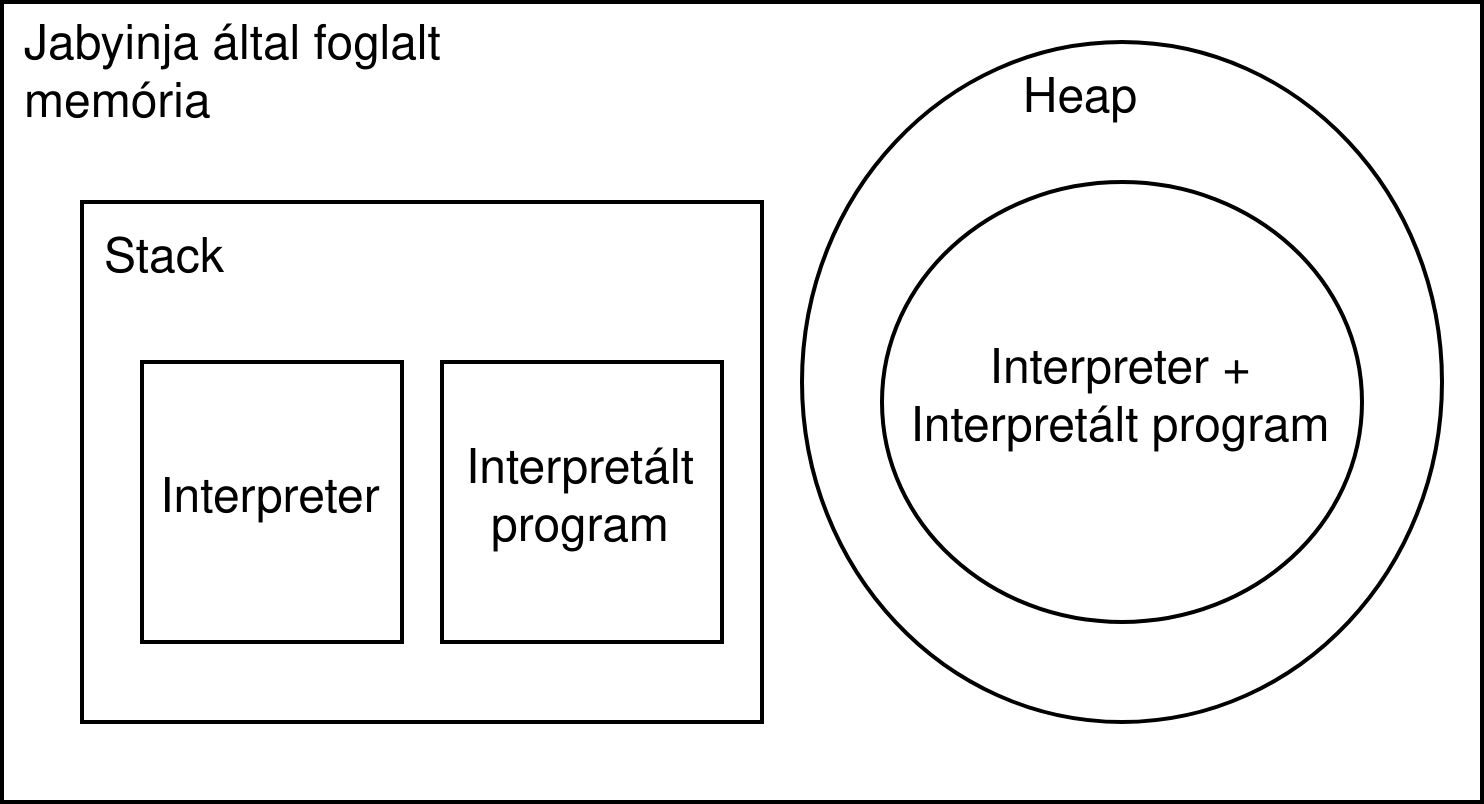
\includegraphics[width=0.6\textwidth,frame]{jabyinja_memory}
	\caption{Jabyinja program memóriamodellje}
	\label{fig:memory}
\end{figure}

\subsubsection{Az önfuttatásról}

Habár a program tényleg képes önmagát lefuttatni, a Java programozási nyelvet mélyebben értő emberek észrevehetik, hogy ez egy erősen kikötéses állítás. Mivel a beépített osztályokat nem interpretálja a program, ezért amikor egy olyan parancsot hívunk meg, mint például: 
\begin{minted}{bash}
$ java -jar target/jabyinja-1.0.0.jar target/classes/com/zoltanbalazs/Main.class target/test-classes/com/zoltanbalazs/PTI/_01/Greet.class World
\end{minted}
akkor igazából csak az interpreter \lstinline{main} metódusáig interpretáljuk azt.

A \lstinline{java} beépített interpreter működése miatt amikor egy jar fájlt futtatunk, az össszes jar fájlban lévő osztály beépített lesz. Az eddig leírtak alapján a beépített osztályok metódusai pedig reflekcióval vannak meghívva.

Természetesen a \lstinline{main} függvényben is megfelelően kell felépíteni a különböző adattagokat, tehát az interpreter tényleg saját magát futtatja, viszont nem látunk akkora erőforrásbeli különbséget mint ami a beépített interpreter és a megírt program között van.

\section{Program szerkezete}

\begin{figure}[H]
	A class fájl beolvasása során a képen látható szerkezeti egység valósul meg a programban. 
	\centering
	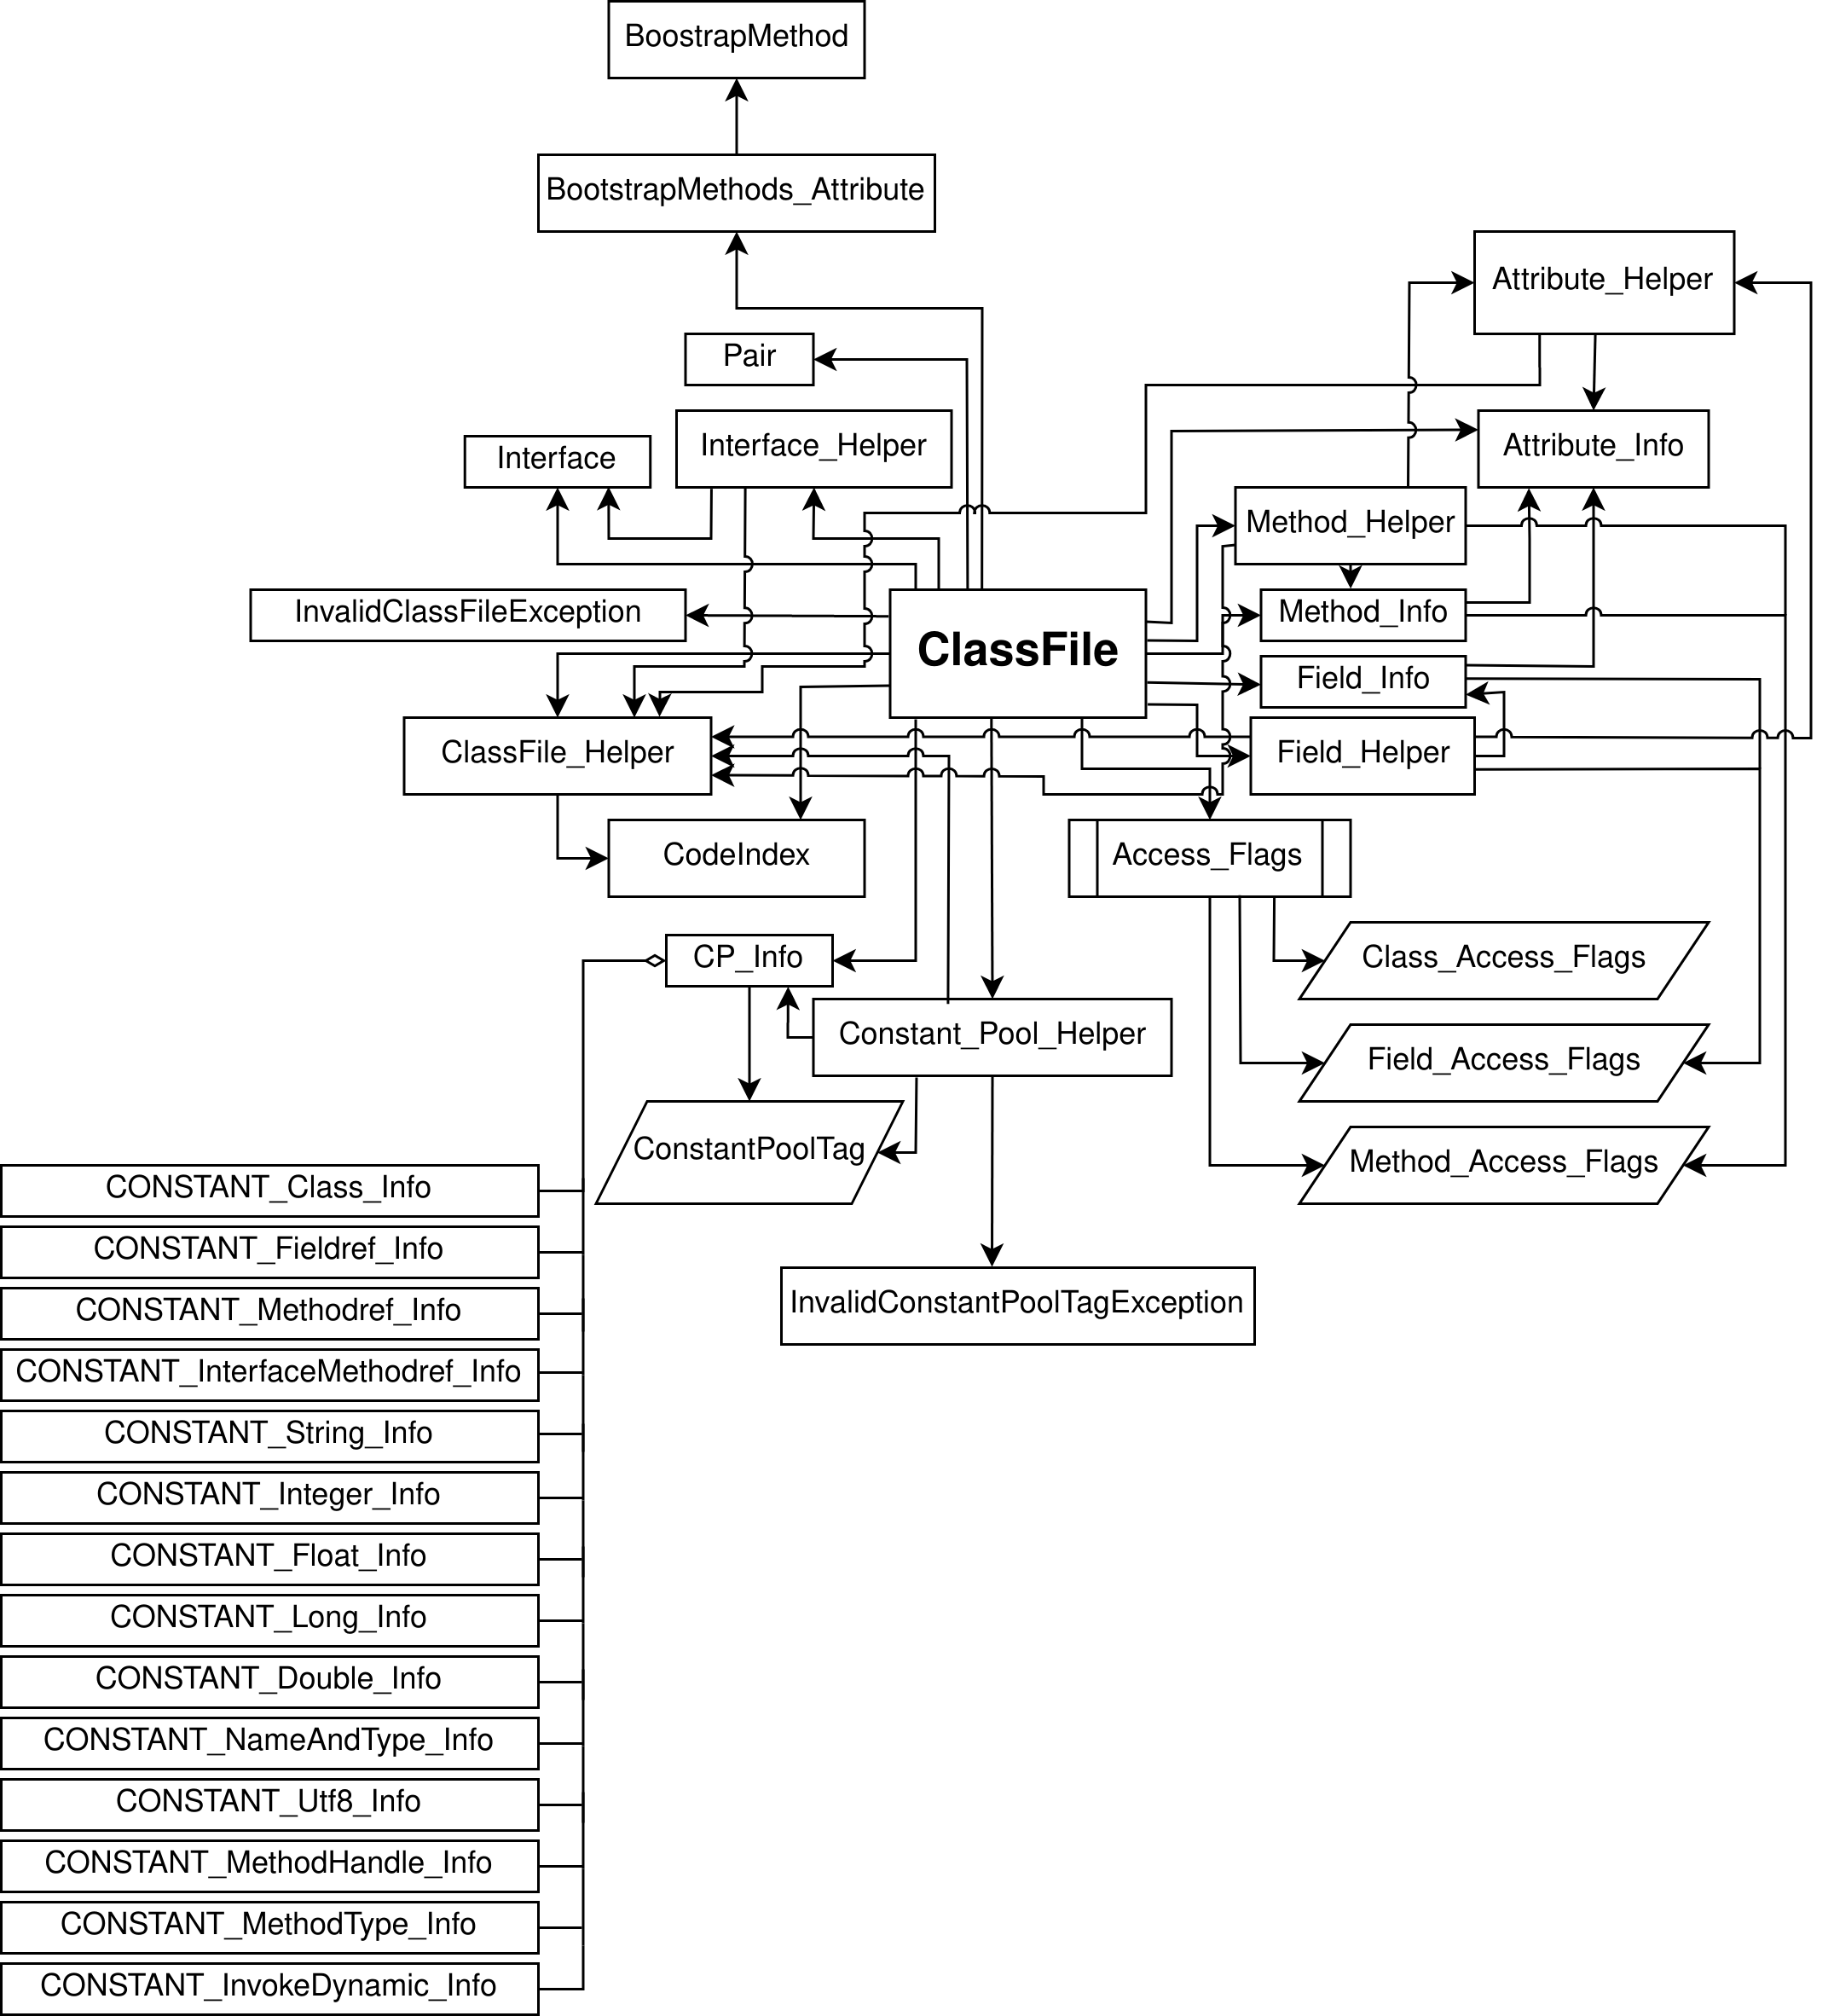
\includegraphics[width=0.9\textwidth,frame]{classfile_diagram}
	\caption{Class fájl beolvasása során a program szerkezete}
	\label{fig:classfile_parse}
\end{figure}

Az ábrán látható, hogy a beolvasás feladata is egy komplex feladat. A különböző segédosztályok viszont megsegítik ennek a kisebb részek való lebontását, azoknak egyszerűbb megértését.

\begin{figure}[H]
	A bájt sorozat értelmezése során a képen látható szerkezeti egység valósul meg a programban. 
	\centering
	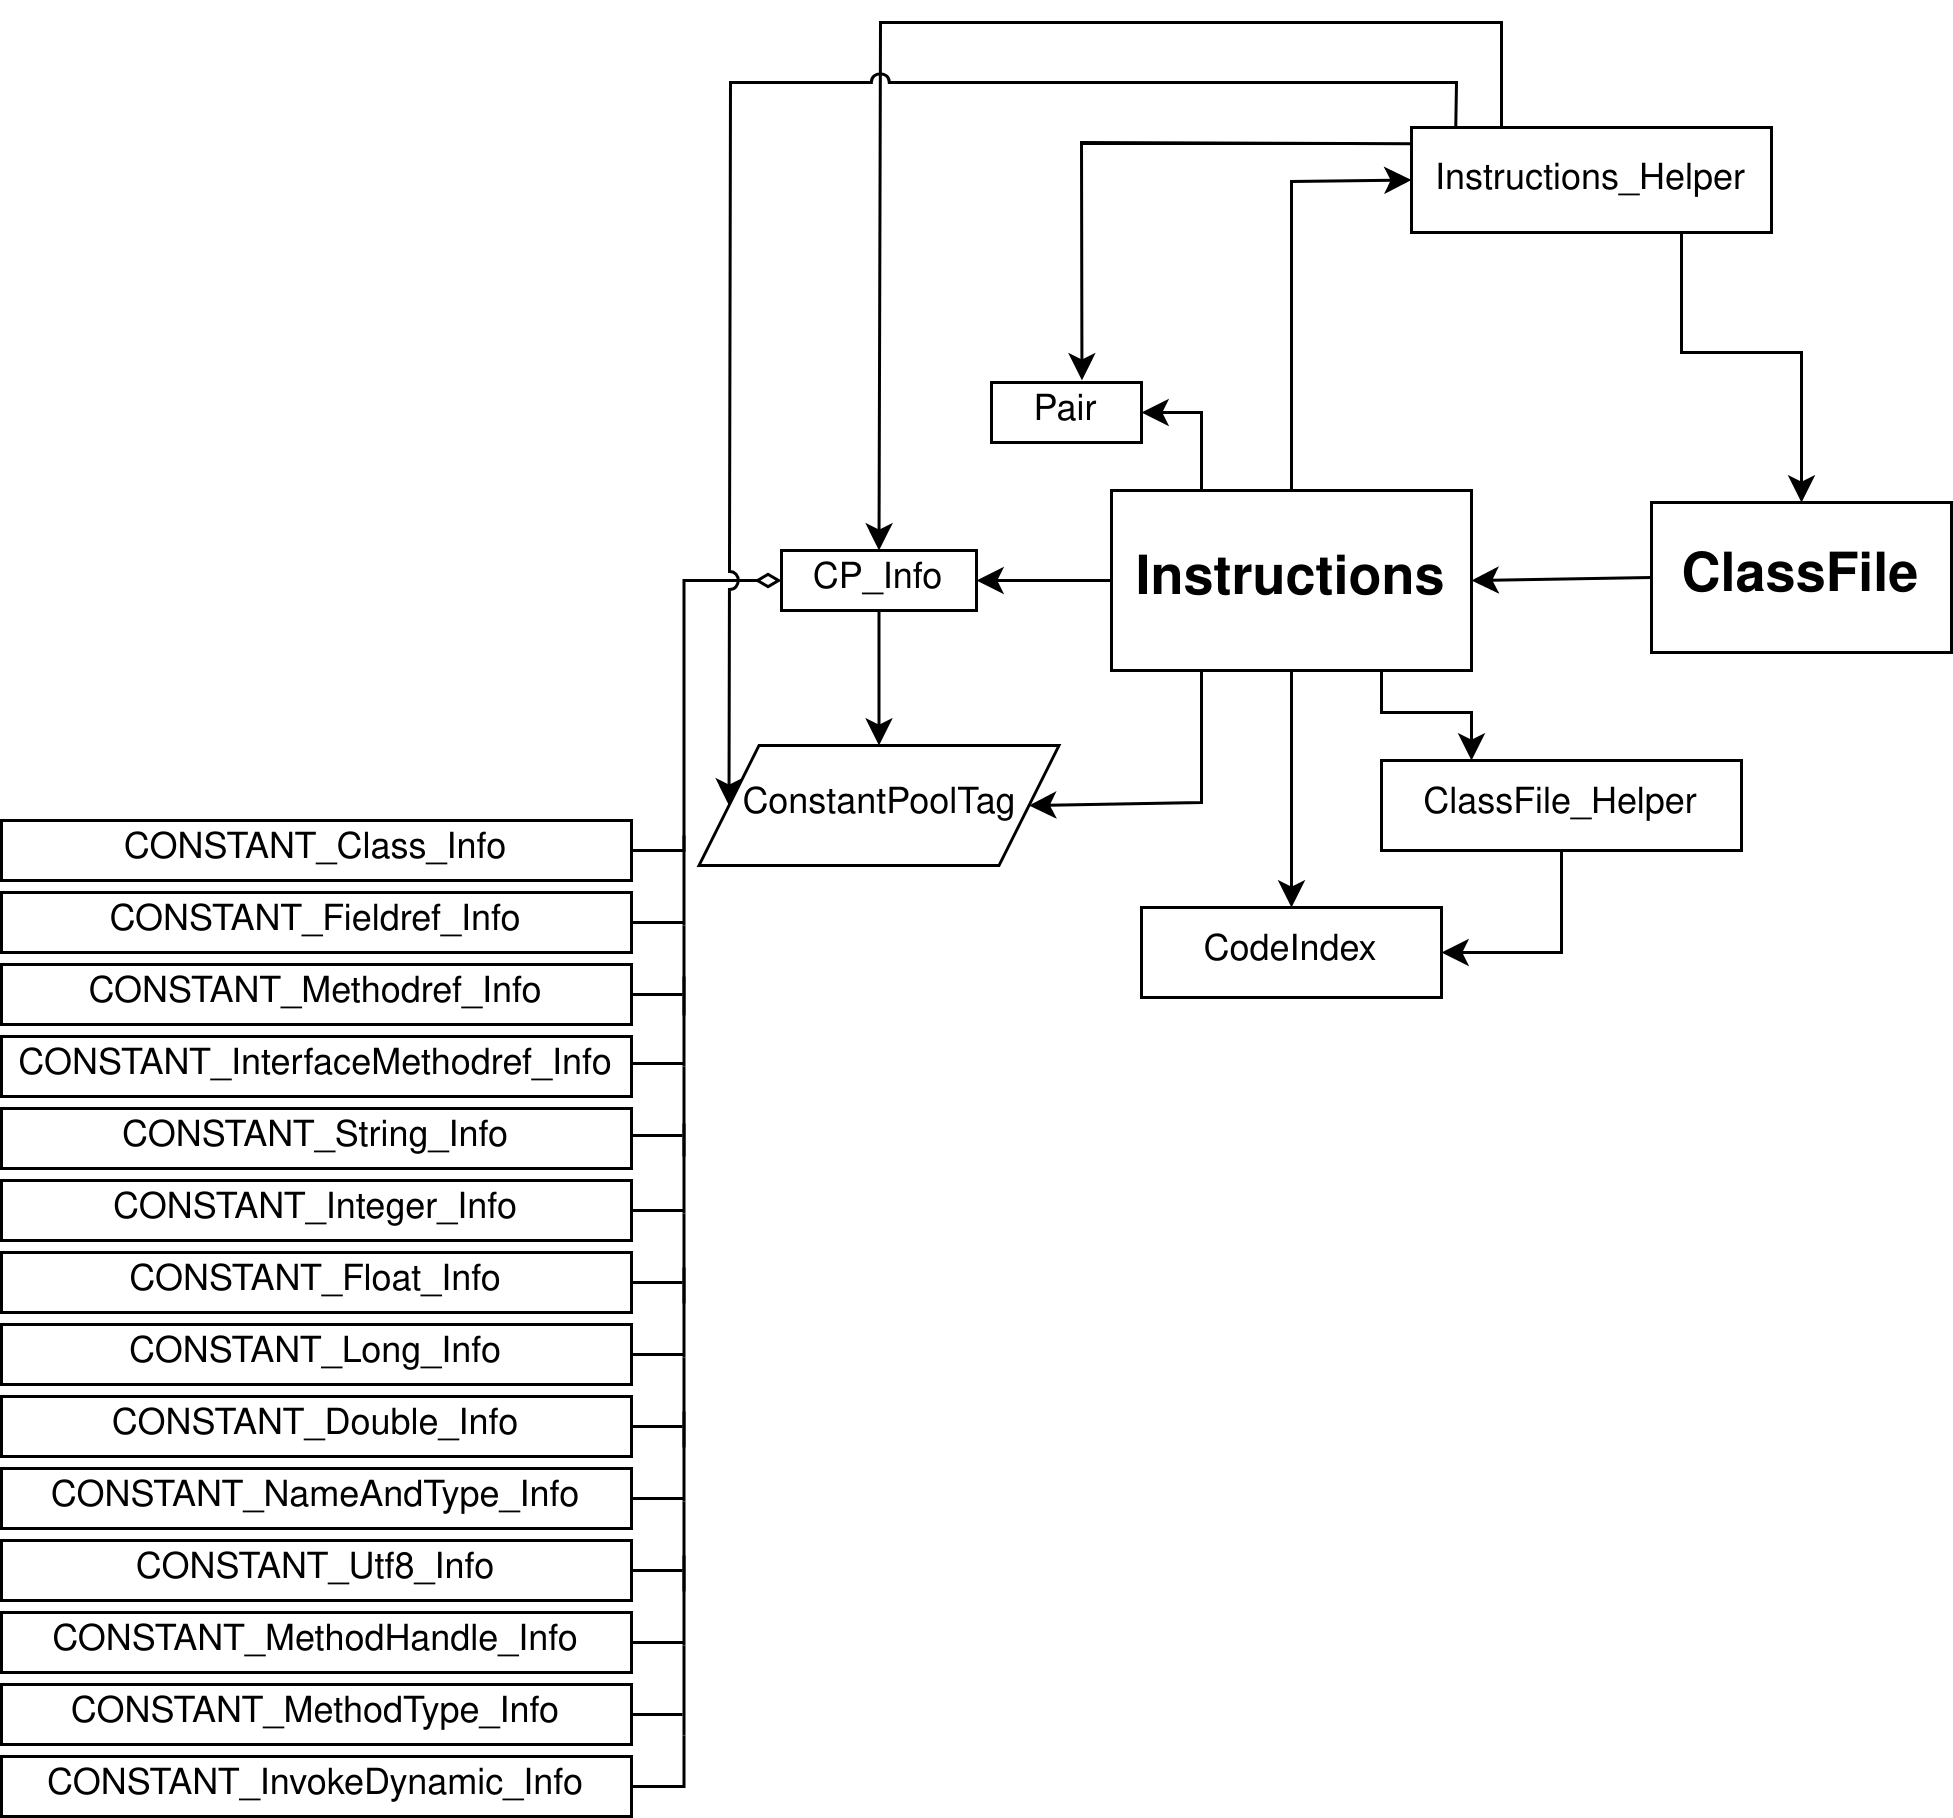
\includegraphics[width=0.9\textwidth,frame]{classfile_execute}
	\caption{Bájt sorozat értelmezése során a program szerkezete}
	\label{fig:classfile_execute}
\end{figure}

Az ábrán látható, hogy némely osztály tagjait nem veszi figyelembe az értelmezés. Ennek oka a reflekció használata, amely során ezen adatokat elhanyagolhatjuk.

\section{Tesztelésről}

A tesztelő környezet egy átlagos Java tesztelő (pl. JUnit) helyett egy saját Python szkript. Az előnye ennek az, hogy a tesztelésnél többet is tud ez a szkript, például a memóriahasználatot és a futási idő különbséget is mérni tudja. A tesztelő szkript a \lstinline{src/test/tester.py} fájlban elérhető. A szkript futtatásához legalább Python 3-as verzió szükséges. A tesztelő működésileg megnézi, hogy a beépített Java interpreter, és a megírt interpreter kimenetei megegyeznek-e, ha igen akkor helyesen fut le az interpret, ha nem, akkor helytelenül. Jelen esetben 3 teszteset van, amelyek nem mennek át a tesztelőn, ezek mindegyike tartalmaz \lstinline{invokedynamic} utasítást.

\subsection{Tesztelés lefuttatása}

A tesztelőt nagyon egyszerűen meg lehet hívni a következő paranccsal:
\begin{minted}{bash}
$ python3 src/test/tester.py
\end{minted}

\textbf{Fontos:} Ha mindegyik teszteset megbukik akkor nincsen fordított állomány! A tesztelő feltételezi hogy jar fájlként van fordítva a program, amely a \lstinline{target} mappában van elhelyezve.

\subsection{Saját teszteset hozzáadása}

Nagyon egyszerűen adható saját teszteset hozzá a szkripthez.
\begin{enumerate}
	\item Helyezzük el a tesztesetet a \lstinline{src/test/java/zoltanbalazs/Own} mappába
	\item Nyissuk meg a tesztelő szkriptet
	\item Adjuk hozzá a megfelelő \lstinline{own_} névvel kezdődő listához a saját tesztesetünket
	\item Ha van, határozzuk meg a bemeneti argumentum(ok) és/vagy standard bemenetről kapott értékek mennyiségét és típusát
	\item A következő futtatásnál az új teszteset le fog futni
\end{enumerate}

\subsection{Tesztelés eredményei}

\begin{figure}[H]
	A teszteket lefuttatva az alábbi eredményt kell kapnunk:
	\centering
	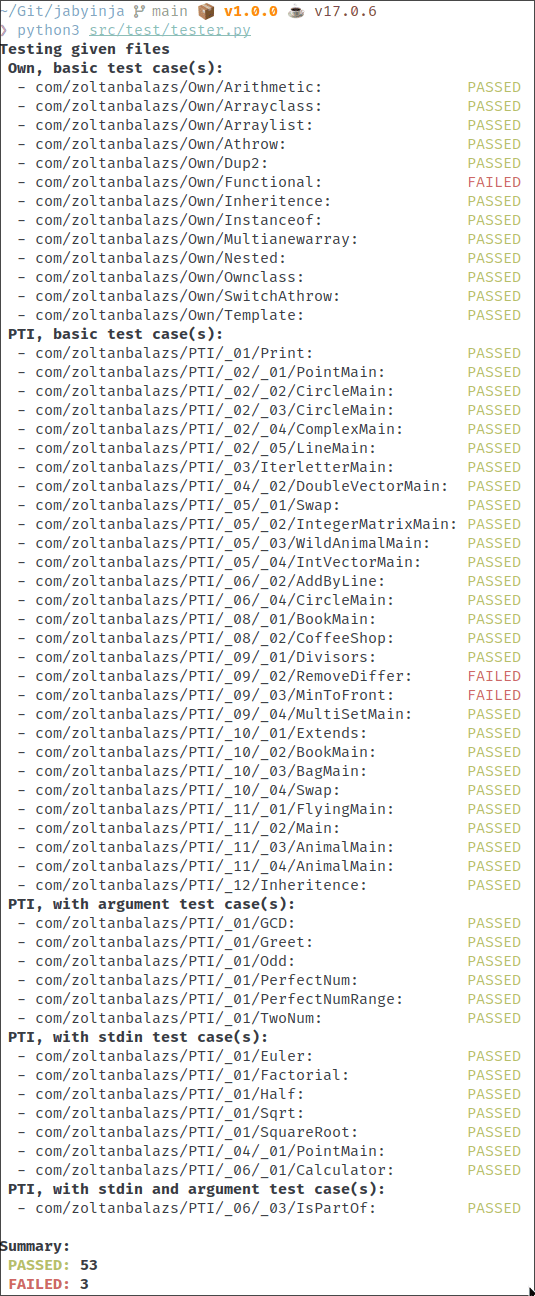
\includegraphics[width=0.6\textwidth,frame]{testing_results}
	\caption{Jabyinja program tesztelésének eredménye}
	\label{fig:testing}
\end{figure}

\section{Továbbiak}

\subsection{Továbbfejlesztési lehetőségek}

\subsubsection{Invokedynamic utasítás}

Az egyik legszembetűnőbb hiány a szakdolgozatban az egyik nem implementált utasítás, az \lstinline{invokedynamic}, hiánya.
Ez az utasítás számos helyen előfordul Java programokban, leginkább a lambda kifejezésekben (ezen belül is a Konkurens programozás tárgyon megismert \lstinline{Executor} osztály paramétereként), illetve a kiírás során szöveg(ek) és változó(k) konkatenációjánál is ez használt.

Az utóbbi egyszerűen kiküszöbölhető a \lstinline{-XDstringConcat=inline} flag-gel való fordítással. Ezen flag használata során az \lstinline{invokedynamic} utasítás lecserélődik \lstinline{StringBuilder}-en keresztül lévő \lstinline{invokevirtual} és \lstinline{invokespecial} hívásokra.

Az előző viszont sajnos jelen állapotban nem megoldott, és nem is oldható meg egyszerűen. Ahhoz hogy lambda függvények működjenek, az \lstinline{invokedynamic}-ot implementálni kell. Ehhez már az alapvető előkészület megvan, a class fájlban lévő \lstinline{bootstrap} metódusok egy külön adattag elemeiként el vannak helyezve. A továbbfejlesztés során csak a megfelelő \lstinline{CallSite} helyet, illetve a class fájlban lévő constant pool általi \lstinline{index}-eken levő metódusokkal (illetve paraméterekkel) kell meghívni az éppen leírt függvényt.

\subsubsection{Java 7 előtti verziók támogatása}

Viszonylag egyszerűen továbbfejleszthető a program hogy Java 7 előtti verzióval fordított class fájlokat is támogasson.

A hiányzó utasítások a \lstinline{ret}, \lstinline{jsr}, \lstinline{jsr_w}, ezek mindegyikéhez csak az szükséges, hogy a megfelelő index-re ugorjunk, a \lstinline{jsr} és \lstinline{jsr_w} utasítások során a visszatérési címet pedig a \lstinline{stack}-re helyezzük.

Természetesen mindegyik utasítás során a megfelelő index-et is be kell olvasnunk a class fájlból, amely a lokális változó megfelelő indexére (\lstinline{ret}), vagy egy adott számot (\lstinline{jsr}, \lstinline{jsr_w}) határoz meg, amely a visszatérési cím, illetve az ugrási cím.

\subsubsection{Optimalizálás}

A futási idő táblázata alapján látható hogy a program exponenciálisan lassabb, mint a beépített \lstinline{java} interpretáló program. A program több memóriát is igényel mint szükséges lenne. Ezeknek számos oka is van, ezek közül pár:

\begin{compactitem}
	\item A nem beépített osztályok megfelelő konstruktorait minden egyes alkalommal a program egyesével keresi ki a program. Ez a limitáció nagyon szembetűnő ha sok saját osztállyal dolgozunk. Ilyenkor a futási idő exponenciálisan lassul. Egy lehetséges megoldás erre hogy a megfelelő konstruktorokat elmenti a program, majd keresés előtt az elmentett konstruktorok között megnézzük hogy szerepel-e már a jelenleg hívandó konstruktor. Ha igen, akkor nem keressük ki, hanem felhasználjuk azt, ha nem, akkor pedig megkeressük.
	\item A \lstinline{local} változóknak maximális értéket ($65536$) foglal a program minden nem beépített függvény meghívása során, viszont a class fájlban ennek a maximális értéke le van írva a megfelelő függvény attribútumaként. Tehát a megoldás erre viszonylag egyszerű; függvényfuttatás előtt kellene a lokális változók mennyiségét beállítani. Ennek a problémának a másik verziója, hogy habár a \lstinline{stack} egy \lstinline{LIFO} (\textit{\textbf{L}ast \textbf{I}n \textbf{F}irst \textbf{O}ut}, amely adat utoljára kerül bele, az kerül elsőnek ki belőle) adatszerkezet, a maximális mérete ennek is a class fájlban a függvény egy megfelelő attribútumaként jelen van. A már megírt függvényekkel viszonylag triviális ezt lekérdezni. (A megfelelő függvény a \lstinline{ClassFile} osztályban található \lstinline{findAttributesByName})
	\item A különböző class fájlok beolvasásának eredménye nincs elmentve, ha egy fájlt be kell olvasnunk, akkor azt minden egyes alkalommal külön-külön megtesszünk. Ha az eredményt elmentenénk akkor drasztikusan lehetne a sebességen gyorsítani. Ennek megoldásaként a \lstinline{Main} osztályban egy listában fel lehetne venni a beolvasott class fájlokat, egy nem beépített class fájlban levő metódus interpretálása előtt pedig végig lehetne menni a már beolvasott fájlokon. Ezzel jóval kevesebb fájl beolvasás műveletet végeznénk, cserébe a listán való végigmenés lehet hogy kevés class fájl használata esetén negatív hatással lenne.
	\item A reflekciót újragondolva, azt elhagyva a sebesség növelhető lenne, erről részletesebben a "Reflekció újragondolása" szekcióban olvashatunk. Lényege, hogy a jelenlegi, beépített osztályokon levő reflekciót le kellene cserélni interpretálása. Az alapok ehhez megvannak, viszont ez is egy komolyabb programozási feladat.
\end{compactitem}

\subsubsection{További tesztelés}

A szakdolgozat írása során megpróbáltam az alapos tesztelésre figyelni, ezért is vannak az alapvető instrukciók egyesével tesztelve (minden tesztfájl-ban külön-külön instrukciók szerepelnek). Viszont a tökéletes program nem létezik, elképzelhető hogy valahol nincs megfelelően a \lstinline{stack} törölve, vagy valamely instrukció mégsem helyes. Ezt a még alaposabb teszteléssel minél inkább meg lehetne cáfolni.

Ehhez egy példa még több tesztfájl mellékelése. A tesztelő környezetbe (Python szkript) viszonylag egyszerűen be lehet helyezni új teszt fájlokat, amely leellenőrzi hogy megfelelő-e a program futása. Továbbfejlesztésként lehet Java programokat írni, majd ezeket a tesztelő környezethez hozzáadni, és ellenőrizni hogy jól lefut-e a program.

Egy másik érdekes továbbfejlesztés, hogy ne csak Java programokat írjunk, hanem más JVM-et felhasználó nyelvekben is írjunk programokat. Ezekkel ellenőrizhetjük hogy a program tényleg képes-e általános Java bájtkódot interpretálni, vagy csak limitált a Java programozási nyelvre. A témabejelentés alkalmával megfogalmazott terveimhez való igazodás miatt az ezekkel a nyelvekkel való tesztelést kihagytam. Egy egyszerű "Hello, World!"-el való tesztelés során (Clojure/Kotlin/Scala nyelven) a program hibát fog dobni. Ennek az indoka a programban levő reflekció, mivel a program Java nyelven van írva, ezért nem találja a Clojure/Kotlin/Scala függvényeket. Helyette érdemes lenne minden egyes fájlt interpretálni, nem csak a nem beépített osztályok fájlait. Természetesen ez megoldható ha a megfelelő nyelv standard könyvtárát be tudjuk másolni a \lstinline{cp} parancssori zászlóval.

\subsubsection{Reflekció újragondolása}

A reflekció egy viszonylag negatív hírrel rendelkező programozási folyamat, melynek számos indoka van. Legtöbbször a reflekció elleni fő indok az, hogy a reflekcióval megoldott problémát valamilyen elegánsabb módon is meg lehetne oldani.

A reflekció túlságos használata miatt a teljesítmény is rosszabb, amelynek javítása egy komoly optimalizálási feladatot eredményez.

A másik komoly probléma a szakdolgozatban a reflekció használatával, a képtelenség arra, hogy Java nyelven kívüli programokat futtatni tudjon. Habár a program készen áll arra, hogy ezeket futtatni tudja, a jelenlegi állapotában nem lehet. Ha minden egyes függvényt interpretálnánk, nem hagyatkoznánk a reflekcióra. Lehetne Java nyelven egy univerzális interpretert írni, amely képes lenne Clojure/Kotlin/Scala fordítóprogramok által generált class fájlokat interpretálni, lefuttatni.

\subsection{Érdekességek a JVM specifikációból}

A specifikációt olvasva számos érdekességre bukkanhat az ember, ezek között vannak tervezési anomáliák, jó megoldások és trükkök. Ezek közül pár:

\begin{compactitem}
 \item A Java 7-es verzió előtt a Java bájtkód instrukciók viszonylag egyszerűek voltak, a 7-es verzióval lett az \lstinline{invokedynamic} bevezetve, mely közelebbi ránézésre igazából egy "szuperinstrukció", ezzel az összes többi \lstinline{invoke} instrukció implementálható, sőt, egy teljes Java bájtkód interpreter is megírható csak \lstinline{invokedynamic} utasításokkal. Az \lstinline{invokedynamic} utasítás a dinamikusság kérdésére volt a válasz. Lényege, hogy azon függvényhívásokat, amelyek paramatéreit fordítási időben nem tudjuk, egy hívási helynek (\lstinline{CallSite}) megfelelően kerülnek a JVM-be bele, amely a hívás során a megfelelő paraméterekkel hívja meg azt.
 \item Elméletileg a lokális változók száma nem kéne hogy $65536$ legyen. Ha megnézi az ember, akkor minden \lstinline{store} és \lstinline{load} utasítás egy darab 8 bites előjel-mentes számot olvas be paraméterként. Ez azt jelenti hogy összesen $2^{8} = 256$ lehetséges index kellene hogy legyen. A \lstinline{wide} módosító utasítás miatt viszont ezek az utasítások beolvashatnak két darab 8 bites előjel-mentes számot, tehát lényegében egy darab 16 bites előjel-mentes szám lesz a paraméterük. Ez azt jelenti hogy $256$ lehetőség hirtelen $2^{16} = 65536$-ra ugrik fel.
 \item Minden \lstinline{Long} és \lstinline{Double} típusú adattag két (egymást követő) helyet foglal el a class fájlon belüli \lstinline{Constant Pool}-ban. Ennek oka hogy minden \lstinline{Constant Pool}-beli elem tényleges felhasználható adata $4$ bájton van, kívéve a \lstinline{Long} és \lstinline{Double}, amelyek felhasználható adatai $8$ bájton vannak. Így a fájlon belüli folytonosság miatt a specifikáció készítői jobbnak látták hogy inkább két helyet foglaljon el. A specifikációban azóta is a "\textit{In retrospect, making 8-byte constants take two constant pool entries was a poor choice.}", magyarul: "\textit{Utólag visszagondolva, rossz döntés volt, hogy a 8 bájtos konstansok két konstans pool bejegyzést igényelnek.}" idézet áll.
 \item A \lstinline{Long} és \lstinline{Double} típusokhoz kapcsolódoan, egy hatalmas különbség a primitívek (\lstinline{double, long}) és osztály (\lstinline{java.lang.Double, java.lang.Long}) típusok között, hogy lokális változókként a primitívek két helyet foglalnak el a lokális változók között; míg az osztály típusok csak egy helyet. Ez azt jelenti, hogyha függvény paraméterként adunk át egy \lstinline{double} primitívet, akkor valójában 2 helyet foglalunk el a lokális változók között, míg ha egy \lstinline{java.lang.Double} értéket adunk át, csak egy 1 helyet fogunk elfoglalni.
 \item A \lstinline{Constant Pool} darabszámára 2 bájt áll rendelkezésre, így maximum $2^{2 * 8} = 65536$ érték szerepelhet a \lstinline{Constant Pool}-ban egy class fájlon belül (ténylegesen a \lstinline{Double} és \lstinline{Long} értékek miatt ez lehet kevesebb). Ez azt jelenti, hogyha különösen nagy a forráskódot tartalmazó fájlunk, akkor lehet, hogy a fordítás során az információ nem fér bele egyetlen class fájlba.
 \item Az előző ponthoz kapcsolódoan, egy függvény maximális paramétereinek száma $2^{16} = 65536$ lehet, mivel a lokális változók darabszámát 2 bájton tárolja el a függvény attribútuma.
\end{compactitem}